\section{Data}
Data is units of information, and in a technical perspective, data is a set
of values of quantitative or qualitative variables about a data object. 
Data should be understood in the context of information. Information can be 
thought of as the resolution of uncertainty, though it's 
exact interpretation and meaning differs in different context. Using this
vague definition of information it becomes clear how diverse data can be.
Everything that removes uncertainty contains information and can potentially 
be stored and processed as data. Examples of data can be 

\begin{itemize}
    \item Tabular Data like spreadsheets.
    \item A news article.
    \item A photograph.
    \item A TV broadcast.
    \item And much much more.
\end{itemize}

Historically, computation has been done on numerical data like tabulated data,
but in the later decades data mining and machine learning methods have broadened
what data algorithms can use to do inference. One example is Neural Networks
and image classification.

\section{Data Mining}
Data mining can be described as:

\begin{center}
    \textit{"Non-trivial extraction of implicit, \\
    previously unknown and potential useful information from data"}
\end{center}

\begin{center}
    \textit{"Exploration and analysis, by automatic or semi-automatic means, \\
    of large quantities of data in order to discover meaningful patterns"}
\end{center}

Data mining is a process of extracting 
and discovering patterns in large data sets involving methods at the 
intersection of machine learning, statistics, and database systems. 
Data mining is an interdisciplinary subfield of computer science and statistics 
with an overall goal to extract information (with intelligent methods) 
from a data set and transform the information into a comprehensible structure 
for further use. \cite{enwiki:datamining}

\section{Machine Learning}

Machine learning can be described as:

\begin{center}
    \textit{"The field of study that gives computers the ability to learn \\
    without being explicitly programmed"}
\end{center}

\begin{center}
    \textit{"A computer program is said to learn from experience E \\
     with respect to some class of tasks T and performance measure P, \\
     if its performance at tasks in T, as measured by P, improves with experience E"}
\end{center}

Machine learning (ML) is the study of computer algorithms that improve 
automatically through experience and by the use of data. It is seen as a part of 
artificial intelligence. Machine learning algorithms build a model based on 
sample data, known as "training data", in order to make predictions or decisions 
without being explicitly programmed to do so. Another way to think about it as 
an abstract mathematical formula.

\begin{equation*}
    f: \text{input} \rightarrow \text{output}
\end{equation*}

The abstract function $f$ can be any regression-, classification-, association
or calculation problem or anything else that can be thought of as the formula
above. In traditional programming, the programmer has collected the input
and manually created $f$ and get the output of interest. I.e. the programmer
collects input, the rules $f$ and calculates the output. In machine learning, 
the programmer have access to the input and the output 
and the computer estimates $f$. I.e. the programmer collects inputs and outputs
and uses the computer to find the rules. 

It should be stated that in some cases output is not used in machine learning. 
There are two different kinds of algorithms, one that learns from outputs called
supervised learning but there are also algorithms that do not learn from data 
tagged by humans but that learn patterns from the data itself.
These are called unsupervised learning algorithms. In those cases a metric or 
criterion is used instead and this is used to learn the rules.
\newpage
\section{Data Mining or Machine Learning}

Data mining is the process of discovering patterns in large data sets involving methods at the interseciton of machine learning, statistics, and database systems.
\begin{figure}[H]
    \centering
    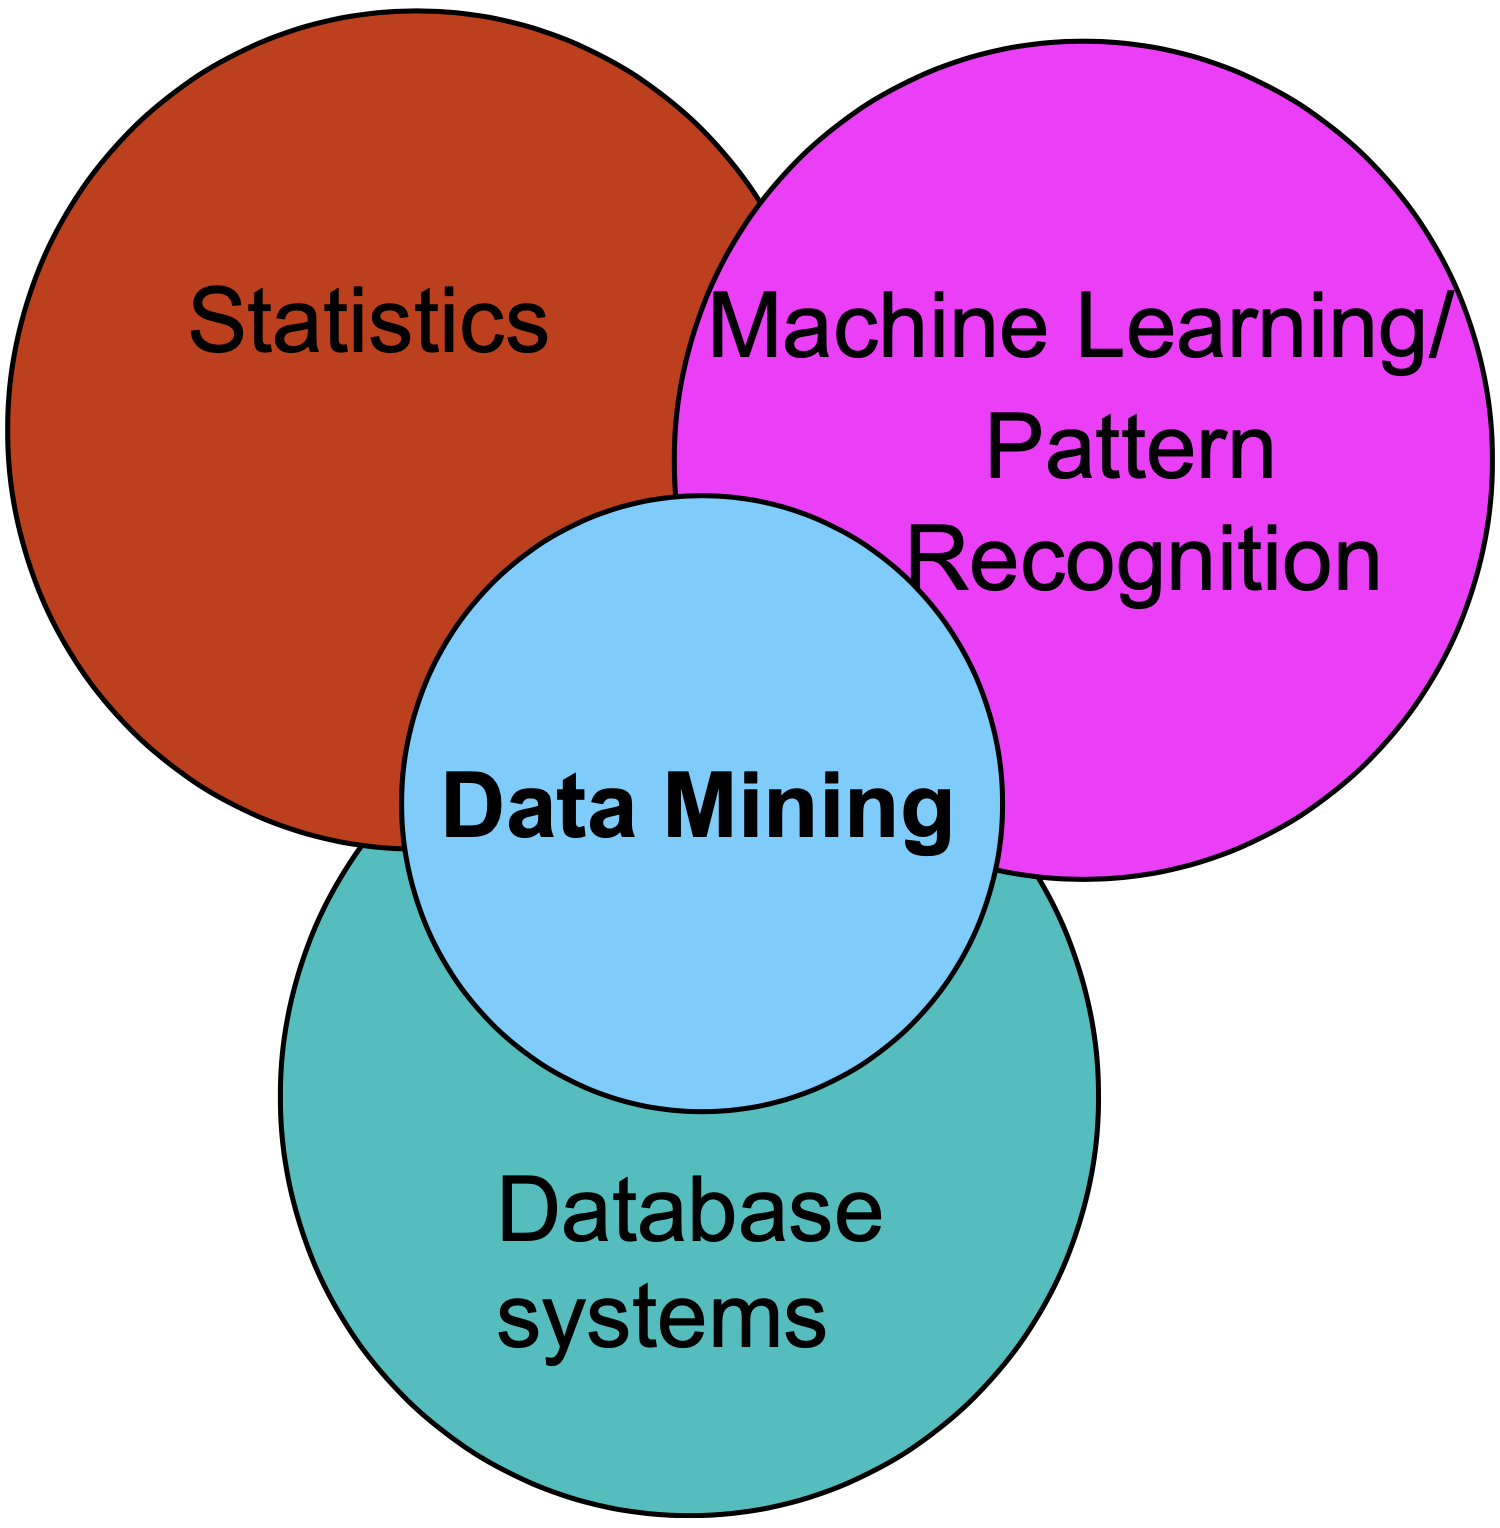
\includegraphics[scale=0.2]{figures/datamining.png}
    \caption{Diagram of Data Mining}
\end{figure}


\section{Data Mining Motivation}

\subsection{Commercial viewpoint}
Lots of data is being collected and warehoused, such as web data, purchases, and transactions.
Computation power has become cheap and powerful, and the competitive pressure is strong.
It is therefore necessary to provide better, customized servicees for an edge.

\subsection{Scientific Viewpoint}
Data is collected and stored at enormous speeds, up to multiple terrabytes per hour.
Such data can be generated from the large hydron collider and from scanning the universe.
Such data can not be interpreted by traditional techniques, and requires data mining to classify and segment the data,
and form hypothesis formations.

\newpage
\subsection{KDD Process}
Knowledge Discovery in Databases (KDD) refers to the overall process of discovering useful knowledge from data.

KDD is an integration of multiple technologies for data management such as database management and data warehousing, 
statistic machine learning, decision support, and others such as visualisation and parallel computing. 

\begin{figure}[H]
    \centering
    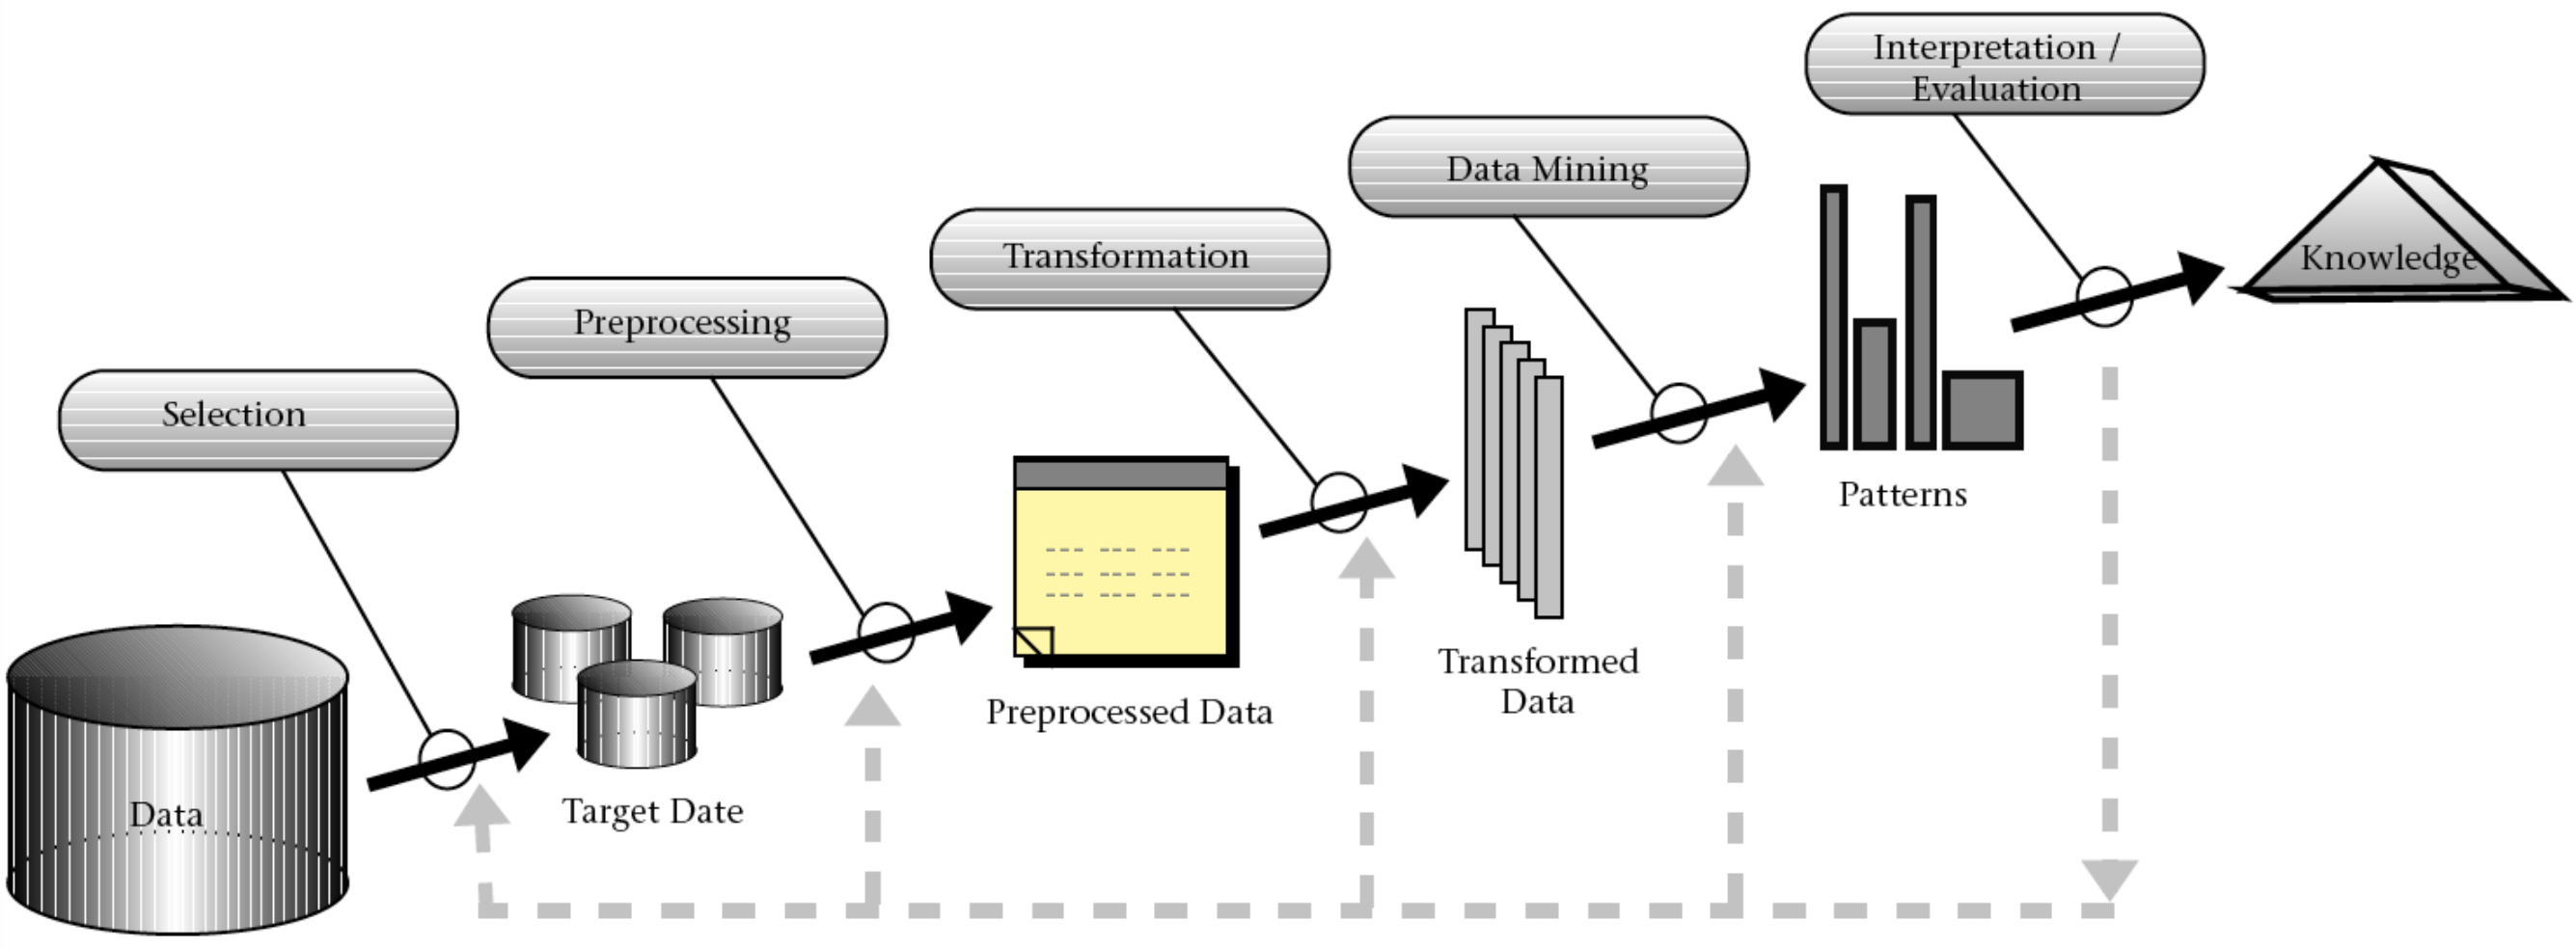
\includegraphics[scale=0.2]{figures/kdd.png}
    \caption{The KDD Process}
\end{figure}

\section{Data Mining tasks}
\begin{itemize}
    \item Prediction methods
    \begin{itemize}
        \item Use some variables to predict unknown or future values of other variables.
        \begin{itemize}
            \item Supervised (classification or regression)
            \item Unsupervised (clustering)
            \item Semi-supervised
        \end{itemize}
    \end{itemize}
    \item Descriptive methods
    \begin{itemize}
        \item Find human-interpretable patterns that describe the data.
        \begin{itemize}
            \item Rule mining
            \item Frequent patterns
            \item Anomaly detection
        \end{itemize}
    \end{itemize}
\end{itemize}
\section{Supervised Learning}
\begin{equation*}
    f: \text{input} \rightarrow \text{output}
\end{equation*}
Supervised learning follow the equation above where it uses the input and
output of example data to estimate the decision function $f$. This is in contrast
with traditional programming where the programmer designed the rules or decision
function $f$ and performed calculations to get an output based on inputs.
Different algorithms in the class of supervised learning are in essence, just 
different ways of estimating $f$. $f$ can have many possible configurations and
parameters and selecting appropriate $f$ estimation methods and tuning the 
correct parameters of $f$ are the main workload in supervised machine learning.
The terminology used in these cases are \textbf{hypothesis space} for $f$ and 
its possible estimation methods and parameters. Constraining the hypothesis 
space must be done to find appropriate algorithms. The parameters that the 
user manually have to change and give as input to the algorithm is called
\textbf{hyperparameters}. They are called such because these are parameters
the model itself does not have access to. The parameters the model itself tune 
we call \textbf{model parameters}. The hypothesis space is therefore the set of
hyperparameters and model parameters. 

\section{Unsupervised Learning}
\begin{itemize}
    \item Unsupervised learning includes unlabeled data
    \item One way of doing this would be to cluster data into to groups
    \begin{itemize}
        \item Group data points which are similar together, while separating 
        dissimilar items as much as possible
        \item This is a clustering algorithm
    \end{itemize}
\end{itemize}

Unsupervised methods does not have the luxury of having the labels of the data,
either because there is no natural labelling or because the data has not yet
been labeled. These methods must use other metrics than labels to estimate the
the decision function $f$. 

\section{Classification}

Given a population $P$ with subpopulations $Y$ and a set of attributes for 
each object in the population $X$, a decision function $f$ must be estimated 
that is able to capture the true state of nature and correctly identify
the correct subpopulation of each object. 

\begin{equation*}
    f: \underset{X \in P}{X} \rightarrow Y
\end{equation*}

\section{Regression}
\begin{enumerate}
    \item Given a set of data points/instances along with “correct” answers or 
    labels (training data)
    \item Feed it to an algorithm which can learn a model and predict the 
    correct value for an unseen data point (test data)
    \item The learned model is an approximate representation of the training 
    data
    \item Predict continuous valued output (price in the previous example)
    \item The algorithm should produce more right answers (goal)
\end{enumerate}

Given a continious variable $X$ with another continious variable $Y$ 
amd a set of observations $D$, a decision function $f$ must be estimated 
that is able to capture the true state of nature and correctly use $X$ to 
predict the corresponding value of $Y$.  

\begin{equation*}
    \underset{X,Y \in D}{f: X \rightarrow Y}
\end{equation*}

\section{Association Rule Mining}
\begin{itemize}
    \item Given a set of records each of which contain some number of items from a given collection
    \item Produce dependency rules which will predict occurrence of an item based on occurrences of other items
\end{itemize}
Such rules can be used for marketing and sales promotion. Rule mining can also be used for inventory management, and much more.

\section{Challenges in Data Mining}
\begin{itemize}
    \item Scalability
    \item Dimensionality
    \item Heterogenous or complex data
    \item Data ownership and distribution
    \item Privacy concern
    \item Data quality
    \item Evolving/streaming data
\end{itemize}
